% References
% https://tex.stackexchange.com/a/331008
% https://tex.stackexchange.com/a/42728
% https://tex.stackexchange.com/a/57745 (accented chars)

\documentclass[twoside,11pt]{article}
\usepackage{amsmath, amsfonts,amsthm,fullpage}
\usepackage{algorithm}
\usepackage{algpseudocode}
\usepackage{graphicx,subcaption,titlesec}
\usepackage{multicol}
\usepackage{multirow}
\usepackage{tabularx}
\usepackage[colorlinks=true]{hyperref}
\usepackage{graphicx,booktabs,array}
\usepackage{changepage}
\usepackage{empheq}
\usepackage{longtable}
\usepackage{tikz}
\usepackage{fontawesome}
\usepackage{csquotes}
\usepackage{adjustbox}

%Add circles to things. Good for inline lists
\newcommand*\circled[1]{\tikz[baseline=(char.base)]{
            \node[shape=circle,draw,inner sep=1pt] (char) {#1};}}

% Adds additional colors. Here's a reference:
% https://www.overleaf.com/learn/latex/Using_colours_in_LaTeX
%\usepackage[dvipsnames]{xcolor}

\usepackage[margin=0.75in]{geometry}
\setlength{\parindent}{0em}
\setlength{\parskip}{0.5em}
\setcounter{secnumdepth}{4}
\renewcommand{\familydefault}{\sfdefault}

% Rename the TOC title
\renewcommand{\contentsname}{Table of Contents}

% =============================================================

\begin{document}
\raggedbottom

% =============================================================

\begin{center}
\Huge{{\textbf{A Collaborative Filtering-based Approach to Patient Journey Mapping and Disease Prediction}}}
\end{center}

\vspace{2em}

\begin{center}
	by

	\vspace{1em}

	\textbf{Nikhil Anand}, \textbf{William Lam}, and \textbf{Shrea Shyam}
\end{center}

\vspace{5em}

\begin{adjustwidth}{100pt}{100pt}
	\small{A Practicum Report submitted to the Department of Industrial and Systems Engineering and the School of Computer Science in Partial Fulfillment of the Requirements for the Degree of Master of Science in Analytics}Ï

	\vspace{2em}

	\begin{center}
		\small{at the}

		\small{\textbf{GEORGIA INSTITUTE} \textit{of} \textbf{TECHNOLOGY}}

		\small{December 2022}
	\end{center}
\end{adjustwidth}

\vfill

\begin{figure}[H]
	\centering
	\includegraphics[width=12em]{images/gatech-seal.png}
\end{figure}

% =============================================================

\newpage

\vspace*{\fill}

\begin{center}
	\textbf{\huge{Executive Summary}}
\end{center}

\begin{adjustwidth}{50pt}{50pt}
\Large{

We were provided anonymized datasets of medical and pharmaceutical claims by our project sponsor \href{https://www.capgemini.com/us-en/}{Capgemini} that detailed over 100,000 patient medical and pharmaceutical records.

We explored a Recommendation Systems-based approach that exploited these datasets to implement an Item-Item Similarity-Based Collaborative Filtering model that would enable an interrogator to

\vspace{1em}

\begin{adjustwidth}{-1.25em}{}
\circled{1} \textbf{Predict conditions} associated with a given condition,
\end{adjustwidth}

\begin{adjustwidth}{-1.25em}{}
\circled{2} \textbf{Chart prospective medical journeys} based on patient similarity,
\begin{adjustwidth}{1.4em}{}
and
\end{adjustwidth}
\end{adjustwidth}

\begin{adjustwidth}{-1.125em}{}
\circled{3} \textbf{Predict the future incidence} of yet unobserved conditions in a 
  \begin{adjustwidth}{1.4em}{}
  given patient.
  \end{adjustwidth}
\end{adjustwidth}

\

Our model may be interrogated via a web application available at \\
\href{https://icd10.ninja}{https://icd10.ninja}

Our code is GNU GPLv3-licensed and may be examined \href{https://github.com/afreeorange/ISYE6748}{on Github}
}

\end{adjustwidth}

\vspace*{\fill}

\begin{center}
	\small{All members contributed equally to this project.}
\end{center}

% =============================================================

\newpage

\tableofcontents

% =============================================================

\newpage

\section{Introduction and Project Goals} \label{section:introduction}

We were provided two datasets that contained anonymized patient medical and pharmaceutical records. We were asked to explore four Use Cases as modeling goals, with the agency to identify any \textit{new} goals that might be of general interest to the overall problems of improving treatment pathways and patient outcomes.


\begin{adjustwidth}{25pt}{25pt}
\textbf{Use Case 1}\\
Which patients are likely to develop a particular illness in the future?

\textbf{Use Case 2}\\
Given a patient who has a set of diagnoses in their history, identify other patients who had a similar history.

\textbf{Use Case 3}\\
Create a chatbot application that can be integrated in a patient self-help portal to direct the queries to the appropriate care manager or caregiver.

\textbf{Use Case 4}\\
Given a discharge summary, extract all the clinically actionable follow-up items in the note.
\end{adjustwidth}


With due consideration to our collective skillsets and the allotted amount of time, we decided to engage \textbf{Use Cases 1 and 2} and re-expressed these cases as \textbf{three key project goals}:
\begin{enumerate}
  \item To \textbf{predict associated disease conditions}

\textcolor{gray}{``I have shingles. What other risks are associated with this condition?"}

  \item To \textbf{help a patient identify other patients with similar conditions} and examine their medical journeys

\textcolor{gray}{``I suffer from shingles and anxiety. Who are \textit{other} people who share my conditions? What \textit{other} conditions do they have?"}

  \item To \textbf{help a patient identify future conditions} based on their current medical disposition

\textcolor{gray}{``I suffer from shingles and anxiety. What other conditions can I \textit{anticipate}?"}

\end{enumerate}

In this report we document our exploration of a hitherto unfamiliar-to-us modeling paradigm (Recommendation Systems) and the results of its application to achieving our stated goals.

\newpage

% =============================================================

\section{The Data}

We were supplied two sets of Parquet files that contained medical and pharmaceutical claims. The list of features in each dataset may be found in Sections \ref{appendix:features:medical} and \ref{appendix:features:pharmeceutical} of the \textbf{Appendix}.

The medical dataset contained 84 features that described 8,092,330 medical encounters of 100,000 patients who could be identified by a unique \texttt{Member Life ID}. 2.41\% (195,498) \texttt{Medical Life ID}s had a value of -1 which we took to indicate missing data.

Similarly, the pharmaceutical claims dataset contained 51 features that described 2,570,133 claims of 54,001 patients who were also assigned a unique \texttt{Member Life ID}. 41.14\% (1,057,426) of patients in this dataset had a \texttt{Medical Life ID}s value of -1.

A union of these datasets on the \texttt{Member Life ID} field was dismaying: it yielded 233 \textit{additional} IDs not present in the medical claims dataset. We assumed that these members had only pharmacy claims and no medical encounters.

The medical claims dataset contained both ICD9 and ICD10 codes. We provide an overview and discuss our choice of the ICD10 system in the next section.

% -------------------------------------------------------------

\subsection{The ICD10 System - Layers, Classes, and Frequencies} \label{section:icd10layers}

The International Classification of Diseases (ICD)\footnote{Originally the ``International Statistical Classification of Diseases, Injuries, and Causes of Death} is a taxonomy of disease classifications that ``contains codes for diseases, signs and symptoms, abnormal findings, complaints, social circumstances, and external causes of injury or diseases"\footnote{Source: \href{https://en.wikipedia.org/wiki/ICD-10}{ICD-10} (\textit{Wikipedia})}. The system is curated by the World Health Organization (WHO) and has evolved through three \textit{versions}: 9, 10, and (as of January 2022) 11. These versions are combined with the ``ICD" abbreviation as ICD9, ICD10, and ICD11 respectively. In the United States, the ICD10 system was adopted as of October 1, 2015 and remains the country's primary medical coding system.

The ICD10 system further specifies \textit{Diagnosis} and \textit{Procedure} code taxonomies\footnote{These are abbreviated to ICD10-CM and ICD10-PCS respectively.}. \textbf{We only dealt with the former} in our analysis: We were only interested in the fact \textit{that} a condition existed and not \textit{how} it was addressed.

Disease classifications within a specific ICD version are not immutable: The 2023 update to Version 10 of the system (ICD10) provides 73,639 total classifications\footnote{Compared to $\sim$68,000 ICD10 classifications as of 2019} of disease conditions\footnote{Source: \href{https://www.cms.gov/medicare/icd-10/2023-icd-10-cm}{The Centers for Medicare and Medicaid Services}}.

Our dataset contained both ICD9 and ICD10 codes. We excised all ICD9 data and preferred ICD10 codes given that they \circled{1} offered a finer resolution of patient maladies and \circled{2} would help any modeling approach by mitigating issues with improper or ambiguous assignment of disease conditions\footnote{There are $\sim$13,000 ICD9 classifications. \href{https://www.cdc.gov/nchs/icd/icd10cm_pcs_background.htm}{According to the Centers for Disease Control} in the United States: ``\textit{The content [ICD-9] is no longer clinically accurate and has limited data about patients' medical conditions and hospital inpatient procedures, the number of available codes is limited, and the coding structure is too restrictive.}"}.

ICD10 Diagnosis codes are organized into a hierarchy\footnote{Which is expressed via ``chapters" that refer to ``blocks" (e.g. H60 - H95) and ``titles" (e.g. \textit{Diseases of the ear and mastoid process}). We are not going to use those terms in our report.} that is (based only on our cursory examination) at most six levels deep\footnote{The WHO offers \href{https://icd.who.int/browse10/2019/en}{a web interface} where one may view this hierarchy (last updated in 2019).}. Here's an example of where a specific disease condition ``Lymphocytic colitis" lies in the  ICD10 hierarchy, with each condition's \textcolor{orange}{ICD10 code/``\textbf{class}"} and \textbf{our custom assignment} of ``\textcolor{cyan}{\textbf{Layer}}" numbers for each hierarchical level:

\


\textcolor{cyan}{Layer \circled{1}} Diseases of the digestive system \textcolor{orange}{[K00-K95]}

\textcolor{cyan}{Layer \circled{2}}\hspace{1em} $\rightarrow$ Noninfective enteritis and colitis \textcolor{orange}{[K50-K52]}

\textcolor{cyan}{Layer \circled{3}} \hspace{2em} $\rightarrow$ Other and unspecified noninfective gastroenteritis and colitis \textcolor{orange}{[K52]}

\textcolor{cyan}{Layer \circled{4}}\hspace{3em} $\rightarrow$ Other specified noninfective gastroenteritis and colitis \textcolor{orange}{[K52.8]}

\textcolor{cyan}{Layer \circled{5}} \hspace{4em} $\rightarrow$ Microscopic colitis \textcolor{orange}{[K52.83]}

\textcolor{cyan}{Layer \circled{6}} \hspace{5em} $\rightarrow$ Lymphocytic colitis \textcolor{orange}{[K52.832]}

\


In the supplied datasets, we observed ICD10 codes at all Layers. However, we  \textbf{chose to restrict our analysis to Layers 1, 2, and 3} in the interest of generating relatively smaller matrices to quickly validate our modeling approach\footnote{Note that even with this three-layer restriction, the ICD10 system still offers a relatively finer resolution of disease conditions (1,914) than ICD9 (1,042) at Layer 3.}. As we will discuss in the ``\hyperref[section:data-prep]{Data Preparation}" section, our decision to limit our analysis to just the top three Layers was also motivated by the fact that patient data naturally gets \textit{sparser} with an increasing level of layer specificity. Table \ref{table:icd10classfrequency} shows each layer's corresponding class frequencies.

\

\begin{table}[H]
  \centering
  \begin{tabular}{|l|r|}
      \hline
    \textbf{Layer} & Number of \textbf{Classes} \\
    \hline
    \hline
    1 & 22 \\
    \hline
    2 & 283 \\
    \hline
    3 & 1,914 \\
    \hline
    4 and below & 71,420 \\
       \hline
  \end{tabular}
  \caption{ICD10 Class frequencies at various Layers}
  \label{table:icd10classfrequency}
\end{table}

There were a total of 51,705 total codes in our raw medical claims dataset which captured $\sim$70\% of all 2023 ICD10-CM Codes.

% -------------------------------------------------------------

\subsection{Note on Terminology}

In this report,
\begin{itemize}
	\item A ``\textcolor{cyan}{\textbf{Layer}}" refers to any one of the numbered hierarchies illustrated by example in the previous section.
  \item ``\textcolor{orange}{\textbf{Codes}}" and ``\textcolor{orange}{\textbf{Classes}}" are synonymous. They refer to ICD10 codes at any \textcolor{cyan}{Layer}.
  \item ``Frequency" and ``Incidence" are synonymous. They refer to the number of times a \textcolor{orange}{Class} was observed in a patient's history of medical encounters at any \textcolor{cyan}{Layer}.
  \item ``Patients" and ``Members" are synonymous.

\end{itemize}

\newpage

% -------------------------------------------------------------

\subsection{Feature Selection}

We attempted to select features based on the domain expertise of a team member who is an experienced former medical coder. However, we will refrain from detailing the process and the many challenges we faced with evaluating and selecting features. This is for the simple reason that our entire feature selection effort was rendered completely unnecessary and futile as our project evolved to employ Item-Item Similarity Based Collaborative Filtering as our model.

As we will explain in the next section, this approach is content-agnostic and does not entail any feature-space requirements. Hence, we dropped \textit{all} features \textit{except} for the \texttt{Member Life ID} and created three ICD10 Code/Class frequency matrices based on patient encounters. We describe these matrices in Section \ref{section:data-prep}.

% =============================================================

\section{The Model}

\subsection{Recommendation Systems}

We identified Recommendation Systems (also called ``Recommender Systems" or simply ``RecSys") as the most suitable approach to realize our project goals. These systems are well-studied\footnote{They were \href{https://en.wikipedia.org/wiki/Recommender_system\#History}{first (unwittingly) identified in 1979}.} and are typically and widely used by companies like Netflix, Spotify, and Amazon to provide product recommendations to their customers. It is safe to state that, at these companies, Recommendations Systems assume a mission-critical importance in terms of how their efficacy drives platform and product engagement\footnote{See: \href{https://en.wikipedia.org/wiki/Netflix_Prize}{The Netflix Prize}}.

A Recommendation System entails three essential entities: a \textbf{User}, an \textbf{Item}, and a user's \textbf{Rating} of an item. It fundamentally considers two sets of \textbf{similarities}\footnote{The word denoting exactly what a reasonable person would think it means.} based on rating, one between users (``user-user similarity") and another between items (``item-item similarity"), to predict how a user \textit{would} rate an item they are yet to interact with.

A canonical example would be a dataset that contained a 0-5 rating of various movies (items) by customers (users)\footnote{Indeed, a lot of tutorials and books on applied Recommendation Systems employ the freely available \href{https://movielens.org/}{MovieLens} dataset as a pedagogical resource. It is published and maintained by the University of Minnesota.}: How would a user who rated ``\textit{Norbit}" 1/5, ``\textit{Bahubali}" 3/5, and ``\textit{Pather Panchali}" 5/5 rate the Kurosawa movie ``\textit{Sanjuro}"? What other movies would this user be interested in? Who are other users who share this user's taste?

\newpage

We argue that Recommendation Systems provide a very elegant mapping from the space of product recommendations to the space of disease condition predictions. Figure \ref{fig:recsys-mapping} illustrates our conception of this mapping with an example.

\begin{figure}[H]
\centering
	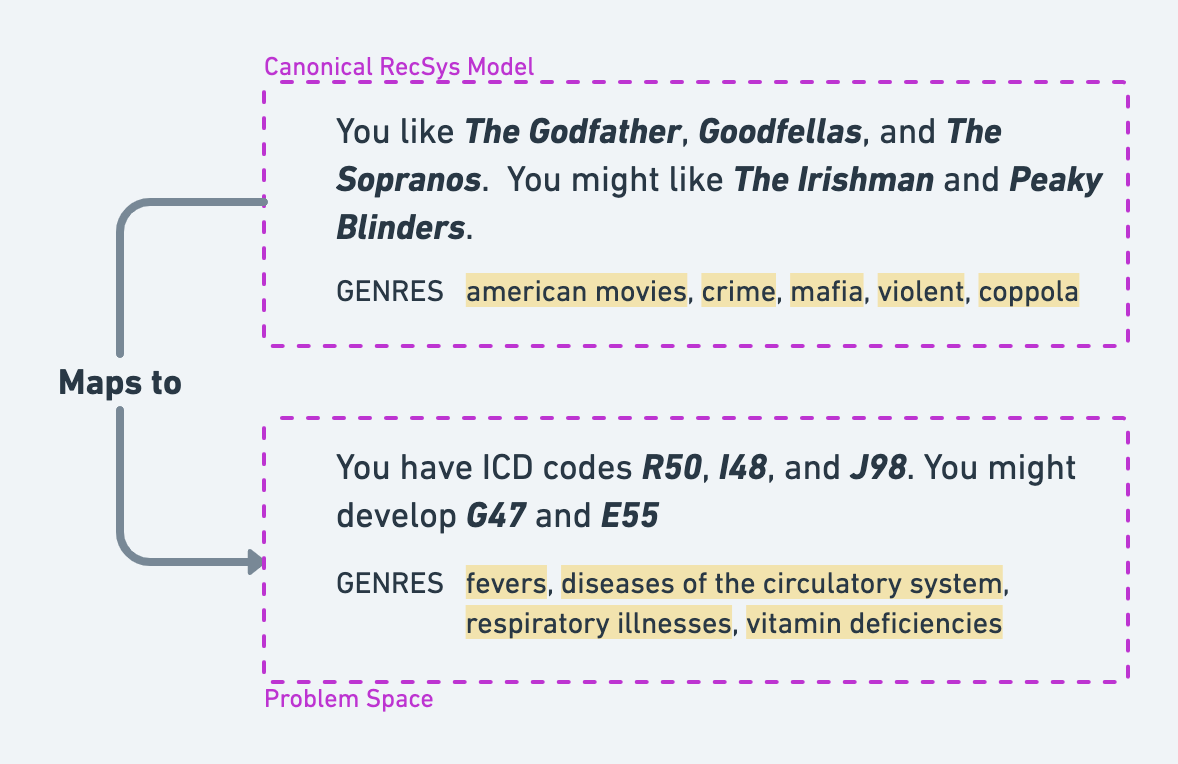
\includegraphics[width=1\textwidth]{./images/recsys-mapping.png}
	\caption{Recommendation Systems map elegantly to the problem of disease condition prediction}
	\label{fig:recsys-mapping}
\end{figure}

In our application of Recommendation Systems,

\begin{itemize}
  \item \textbf{Users} $\xrightarrow[\text{to}]{\text{Map}}$ \textbf{Patients} with unique \texttt{Member Life ID}s

  \item \textbf{Items} $\xrightarrow[\text{to}]{\text{Map}}$ \textbf{ICD10 Classes} at each layer \\ E.g. ``A00-B99" at Layer 1, ``K35-K38" at Layer 2, and ``Q23" at Layer 3

  \item \textbf{Ratings} $\xrightarrow[\text{to}]{\text{Map}}$ Observed \textbf{Class Frequencies} \\This is simply the number of times a given patient's encounter was labeled with an ICD10 Class. E.g. How many times did a patient with \texttt{Member Life ID} 154 get assigned a diagnostic code H40 (Glaucoma)?
\end{itemize}

The `genres' in Figure \ref{fig:recsys-mapping} would map to the \textit{feature-space representation} of each ICD10 Class which we will discuss shortly.

% -------------------------------------------------------------

\subsubsection{Determining Similarity} \label{section:similarity}

For a basic Recommendation System implementation, we need to define a Similarity Function $S$ that provides us a continuous real-valued response to the `closeness` of two input vectors. This function may then be used to construct two square \textit{similarity matrices} that contain pairwise user-user and item-item similarities.

We explored commonly used similarity metrics like Jaccard Distance (which was inapplicable given that it would collapse Class frequencies $f\in\mathbb{Z}$ into $f\in\{0,1\}$ leading to a loss of information and resolution) and L1 and L2 distances (which only consider absolute values and subsume directionality\footnote{Consider three simple vectors $a = [1,1,0,1]$ $b = [1,0,1,1]$ and $c = [1,0,0,0]$. Euclidean similarity (which is $1 - Distance$) between $\{a \leftrightarrow b, b \leftrightarrow c, c \leftrightarrow a\}$ would be exactly the same at $\{-0.414, -0.414, -0.414\}$. However, the Cosine Similarities would be $\{0.667, 0.577, 0.577\}$ which evidently allow for a better differentiation between the vectors.}). Note that $k$-means clustering is a `higher-order' method that can employ any similarity metric for classification.

We settled on the the commonly-used Cosine Similarity as our choice of $S$. If $u$ and $v$ are two vectors (of users or items),

\begin{equation}
  S(u, v) = cos(\theta) = {\mathbf{u} \cdot \mathbf{v} \over \|\mathbf{u}\| \|\mathbf{v}\|} \in [-1, 1]
  \label{eq:similarity-cosine}
\end{equation}

Intuitively, this metric measures the angle $\theta$ between vectors $u$ and $v$: smaller values of $\theta$ imply greater similarity.

Cosine Similarity in Recommendation Systems is typically either \textit{Centered} around the mean of the vector\footnote{In which case it becomes the familiar Pearson Correlation Coefficient.} or \textit{Normalized} to $[0,1]$ using the vector's minimum and maximum values. We evaluated three variants: Unadjusted, Centered, and Normalized.

We used our similarity function to create six matrices for $m$ patients, $n$ ICD10 Classes, and three Layers $l \in \{1,2,3\}$
\begin{itemize}
  \item The matrices ${}^{l}P$ contained pairwise patient-patient similarities which were computed using $S(u, v)$ based on observed class frequencies for Layers 1, 2, and 3. They have a dimension $m \times m$.

  ${}^{l}P_{ij}$ denotes the similarity between patients $i$ and $j$ based on their observed ICD10 Class frequencies at layer $l$

  \item Conversely, the matrices ${}^{l}C$ contain pairwise ICD10 Class frequency similarities for a given Layer based on the number of patients who were observed for that class. They have a dimension $n \times n$.

  ${}^{l}C_{ij}$ denotes the similarity between ICD10 Classes $i$ and $j$ based on their observed incidences across patients at layer $l$.

\end{itemize}

% -------------------------------------------------------------

\newpage

\subsubsection{Filtering in the Neighborhood} \label{section:filtering-in-n}

In Recommendation Systems, a \textit{neighborhood} is defined as the subset of top-$n$ entities (users or items) that are similar to each other. \textit{Filtering} is the act of performing ratings predictions within this subset. There are three approaches to filtering: Content, Collaborative, and a Hybrid of both. Figure \ref{fig:recommender-systems} provides a visual summary and highlights our approach.

\begin{figure}[H]
  \includegraphics[width=\textwidth]{./images/recommender-systems.png}
  \caption{A visual summary of Recommendation Systems. Our final approach was Collaborative Filtering in the Neighborhood based on item-item similarity.}
  \label{fig:recommender-systems}
\end{figure}

In this section we will offer a very brief overview of Content and Collaborative filtering approaches, their pros and cons, and explain our choice of Collaborative Filtering as the candidate approach.

\

\textbf{Content Filtering}

\vspace{2em}

\centerline{``You like X and Y, which are things like A, B, and C.
So you might like Z which is like A, B, and C."}

\vspace{1em}

Here, X and Y are items, and A, B, and C are the \textit{features} of these items.

For instance, if you like `X = Siberian Husky` and `Y = German Shepherd`, the features might be `A = Shedding Coat`, `B = Large-to-Medium Size`, `C = Working Breed` (all binary variables in this example). The set of all features $\{A, B, C,...Z\}$ comprises the \textit{feature-space} of puppy attributes.

Endowed with a robust feature-space, Content Filtering's biggest advantage is its ability to provide a user ($\leftrightarrow$ patient) with an item's ($\leftrightarrow$ ICD10 Class') rating ($\leftrightarrow$ Class frequency) predictions \textit{outside} of \textit{other} users' ($\leftrightarrow$ patients') interactions ($\leftrightarrow$ medical histories/trajectories). Our predictions of future ratings for a given/new user do not depend on recomputing a user-user similarity matrix. However, this is also a downside because of the problem of overspecialization: in its inability to predict out-of-profile conditions, it is incapable of exploiting the trajectories of other users to enhance its predictions. This disadvantage was at odds with a project goal to map patient journeys.

It is also precisely the feature-space requirement that is Content Filtering's main drawback. In our mapping, items are ICD10 Disease Condition Classes, and the construction of a feature-space that encompasses their attributes requires significant medical domain knowledge. It is very laborious to discover and validate both the veracity and completeness of this space for Content Filtering to demonstrate its benefits. This was the biggest disadvantage of Content Filtering to our efforts given the time and domain-knowledge constraints in mapping out the features that correspond to a given ICD10 Class at any Layer.

\

\textbf{Collaborative Filtering}

\vspace{2em}

\centerline{``You like X and Y. People like you like Z. So you might like Z."}

\vspace{1em}

The essential idea of this approach is that users (patients) in a similarity neighborhood who agree on their ratings (number of encounters/ICD10 Class frequencies) of items (ICD10 Classes) are more likely to agree again in the future.

Contrasted with Content Filtering, Collaborative Filtering has a \textit{significant} advantage in that it \textit{does not require a feature-space representation}. This approach is \textit{content-agnostic} and presumes a `generative force' that explains how users (patients) rate (get assigned ICD10 Class frequencies to) items (disease conditions). Domain knowledge is rendered unnecessary here.

This feature of Collaborative Filtering was extremely attractive to us given our stated time and medical domain-knowledge constraints and is the approach we adopted to accomplish a key project goal.

Collaborative Filtering can use \textit{both} the user-user and item-item similarity matrices we built in the ``\hyperref[section:similarity]{Determining Similarities}" section.

% -------------------------------------------------------------

\subsubsection{Cold Starts and First Raters}

If one considers a  matrix of users and items, the ``Cold Start Problem" pertains to the difficulty of predicting ratings for \textit{new users} who have not yet had a chance to offer ratings to \textit{existing items}.  Conversely, the ``First Rater Problem" pertains to the addition of new items: \textit{existing users} have not yet had an opportunity to rate \textit{new items}. These are typical problems with implementing Recommendation Systems.

We posit that \textbf{the Cold Start Problem is inapplicable to our case} as a healthy person (i.e., an individual with no medical encounters) would simply not populate our dataset. The ingress of a new user/patient would be marked by the rating/increase in ICD10 Class frequency of at least one item/disease condition. For hypothetical explorations, the creation of a \textit{synthetic} patient profile by our model's interrogator\footnote{See \hyperref[appendix:websitescreenshots]{the \textbf{Appendix}} for our attempt at enabling the creation of synthetic patient profiles.} obviates this problem\footnote{For example: When Apple Music or Spotify ask you what genres of music you are interested in when you create a new account, this is the precisely problem they seek to solve.}.

We also maintain that the \textbf{First Rater Problem does not apply to our case} since we assume that ICD10 Classes as items are relatively stable classifications, particularly at higher hierarchical levels. They do not grow as rapidly as, say, a collection of books or movies.

For instance, 1,176 codes were added\footnote{Which was an aberration! If we were `upgrading' from 2022 codes, we would see 159 added, 32 deleted, and 20 revised codes.}, 251 codes were deleted, and 36 codes were promoted to some parent class in the 2023 revision of ICD10-CM\footnote{Source: \href{https://www.wolterskluwer.com/en/expert-insights/2023-icd10-code-updates}{Three things to know about the 2023 ICD-10 code updates}, \textit{Wolters Kluwer}}. These updates had zero bearing on our three layer classes. Even if they do in the future, recomputation of item-item similarity is quick and simple as we do not have many items (a few thousand at Layer 3).

% -------------------------------------------------------------

\newpage
\subsubsection{Global, Regional, and Local Effects}

Modern Recommendation Systems do not just rely on Collaborative (or Content, or Hybrid) Filtering to offer recommendations/predictions. As illustrated in Figure \ref{fig:effects}, they are typically tiered into a stack that produces an overall prediction of a user's rating.

\begin{figure}[H]
	\centering
  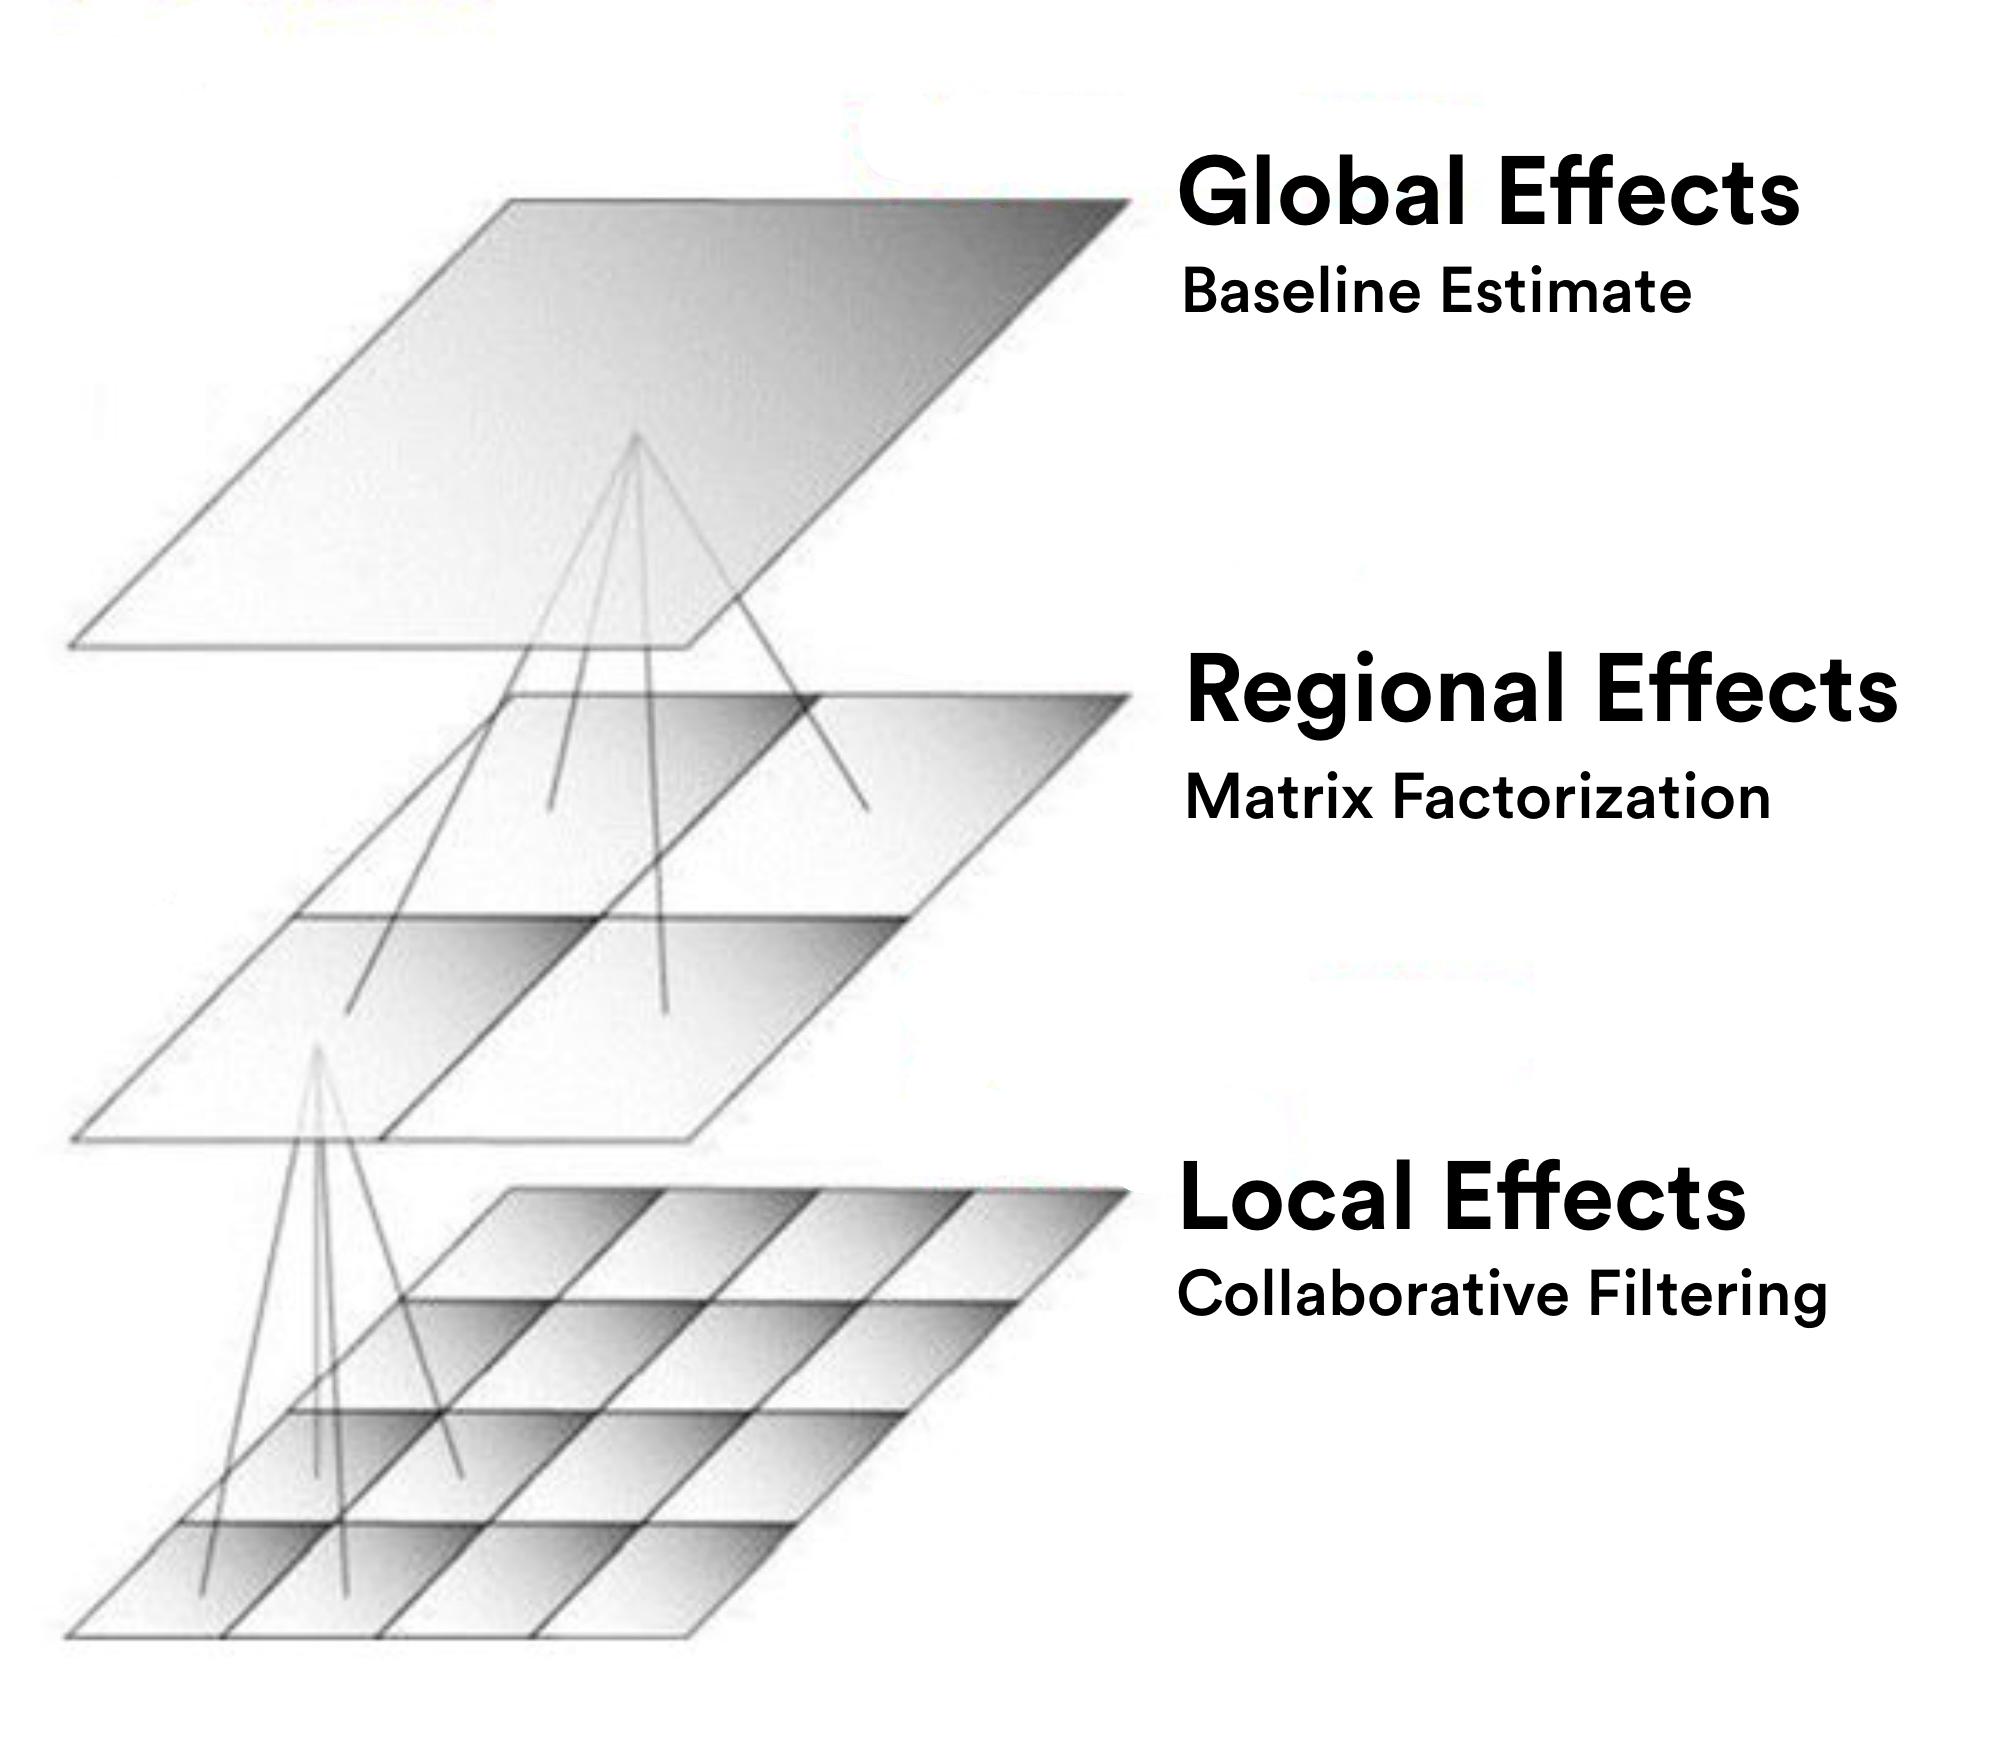
\includegraphics[width=0.7\textwidth]{./images/global-regional-local.png}
  \caption{A modern Recommendation System's Tiers (Image adapted from \href{http://snap.stanford.edu/class/cs246-2015/slides/08-recsys2.pdf}{Jure Leskovec's lecture on RecSys})}
  \label{fig:effects}
\end{figure}

The modeling of \textbf{Regional Effects} typically involves factoring a user-item rating matrix to reveal the underlying structures or generative forces that explain the ratings in the matrix. These structures and forces are variously termed features, concepts, and latent factors depending on the application context. A classic example is factoring a user-item movie rating matrix to reveal genres as features. Some approaches used to model regional effects are Singular Value Decomposition (SVD), Stochastic Gradient Descent (SGD) and Gradient Descent (GD).

We determined that \textbf{regional modeling is inapplicable to our case} because we argue that:
\begin{itemize}
  \item One set of domain experts (the WHO) have already come up with the underlying structures (the features, concepts, and latent factors) of disease expression: This is simply the ICD10 Classification system.
  \item Another set of domain experts (the healthcare providers) have classified patients \textit{into} these structures.
\end{itemize}

In the parlance of Recommendation Systems, ignoring regional effects means that our Collaborative Filtering approach is strictly \textit{memory}-based and not \textit{model}-based\footnote{We will still refer to our approach as a `model' since this distinction is local to Recommendation Systems.}.

This leaves us with applying \textbf{Global Effects}, which can be as simple as \circled{1} Determining the mean of the entire user-item rating matrix and \circled{2} assigning it as the rating prediction.
\newpage
A slightly more sophisticated approach is to consider the \textit{bias} of both users and items in creating a \textbf{Global Baseline Estimate} $b_{xi}$ described by equation \ref{eq:baseline}{.

\begin{equation}
  b_{xi} = \mu + b_x + b_i
  \label{eq:baseline}
\end{equation}

Here,
\begin{itemize}
  \item $\mu$ is the global mean of the user-item rating matrix. \\In our case, this is the mean of all observed Class frequencies for each Layer.
  \item $b_x$ is how much a given user/patient deviated away from the global mean.
  \item $b_i$ is how much the item/ICD10 Class deviated away from the global mean.
\end{itemize}

A quick example: Say the global mean of the frequency of observation for Layer 1 codes is 4.3. A patient with \texttt{Member Life ID} 819 has a mean number of encounters equal to 1.2 (across all classes). This implies that $b_x = (1.2 - 4.3) = -3.1$ (because it is lower than the mean). Assume we are trying to predict this patient's rating/frequency for the Class I00-I99\footnote{Diseases of the circulatory system} and observe that, on average,  patients tend to have 5.9 encounters with this class. This implies that $b_i = (5.9 - 4.3) = 1.6$ (because it is higher than the mean)

Hence, the Global Baseline Estimate for Member 819 for class I00-I99 is $b_{xi} = (4.3 - 3.1 + 1.6) = 2.8$

% -------------------------------------------------------------

\subsection{The Final Model}

We realized our project's goals from the \hyperref[section:introduction]{\textbf{Introduction}} to this report with the choice of Recommendation Systems and Collaborative Filtering as follows:
\begin{enumerate}
  \item To \textbf{predict associated disease conditions}

\textcolor{gray}{``I have shingles. What other risks are associated with this condition?"}

\textcolor{teal}{\faHandORight \hspace{0.25em} Interrogated and ranked the top-$n$ conditions from an item-item similarity matrix ${}^{l}C$ at each level of a condition's rank in the Layer hierarchy. E.g., a Layer 3 condition would receive predictions for \textit{all} Layers 1, 2, and 3. A Layer 2 condition would receive predictions for only Layers 1 and 2.}

  \item To \textbf{help a patient identify other patients with similar conditions} and examine their medical journeys

\textcolor{gray}{``I am Member ID 154 and suffer from shingles and anxiety. Who are \textit{other} people who share my conditions? What other conditions do \textit{they} have?"}

\textcolor{teal}{\faHandORight \hspace{0.25em} Interrogated and ranked the top-$m$ patients from user-user similarity matrices ${}^{l}P$ at \textit{all} Layers.}

  \item To \textbf{help a patient identify future conditions} based on their current medical disposition

\textcolor{gray}{``I suffer from shingles and anxiety. What other conditions should I \textit{anticipate}?"}

\textcolor{teal}{\faHandORight \hspace{0.25em} Combined the Global Baseline Estimate with Item-Item Similarity-Based Collaborative Filtering to predict disease frequencies for a requested ICD10 Class at each Layer for the given patient.}

\end{enumerate}
\newpage
Apropos Goal \#3, and for layer $l \in \{1,2,3\}$, let
\begin{itemize}
  \item ${}^{l}S_{ij}$ be a matrix of similarities. In our case, it is exactly equal to ${}^{l}C_{ij}$ from Section \ref{section:similarity} because we are employing item-item similarity\footnote{Note that one could set ${}^{l}S_{ij} = {}^{l}P_{ij}$ and obtain a user-user similarity-based formulation.}
  \item ${}^{l}N(i; x)$ be the neighborhood of ICD10 Classes that are most similar to $i$ that have been observed in patient $x$ at layer $l$
  \item ${}^{l}f_{xj}$ be the observed frequency of Class $j$ for patient $x$ at layer $l$
  \item ${}^{l}b_{xj}$ be the \textit{local} baseline estimate of the frequency of Class $j$ for patient $x$ at layer $l$
  \item ${}^{l}\mu$, ${}^{l}b_x$, and ${}^{l}b_i$ be the global class frequency mean, bias of patient $x$, and bias of class $i$ at layer $l$
\end{itemize}

We estimate ${}^{l}f_{xi}$ as the predicted frequency of an unobserved class $i$ for patient $x$ at layer $l$ using Equation \ref{eq:model}

\begin{equation}
\begin{align*}
{}^{l}f_{xi}
&= {}^{l}b_{xj} + \frac{
  \sum_{j \in {}^{l}N(i;x)} {}^{l}S_{ij} \cdot ({}^{l}f_{xj} - {}^{l}b_{xj})
 }{
  \sum_{j \in {}^{l}N{i;x}} {}^{l}S_{ij}
 } \\
&= ({}^{l}\mu + {}^{l}b_x + {}^{l}b_{i}) + \frac{
  \sum_{j \in {}^{l}N(i;x)} {}^{l}S_{ij} \cdot ({}^{l}f_{xj} - {}^{l}b_{xj})
 }{
  \sum_{j \in {}^{l}N{i;x}} {}^{l}S_{ij}
 }
\end{align*}
\label{eq:model}
\end{equation}

% -------------------------------------------------------------

\subsection{Preparing Data for The Model} \label{section:data-prep}

If $U$ is the set of all patients and ${}^{l}I$ is the set of all ICD10 Classes at layer $l \in \{1,2,3\}$, we defined a utility matrix ${}^{l}M \gets U \times {}^{l}I$ where ${}^{l}M$ is a totally ordered set\footnote{We note this fact as an aside. The properties of the utility matrix only assume importance when one attempts its factorization.} that contains the encounter frequencies of classes ${}^{l}I$.

We prepared these three utility/frequency matrices for each layer by \textbf{aggregating ICD10 code assignments from medical encounters} from the original medical claims dataset into Layer 1, 2, and 3 classes which were established based on \href{https://www.cms.gov/medicare/icd-10/2023-icd-10-cm}{2023 ICD10-CM data obtained from the Centers for Medicare \& Medicaid Services} (i.e. we did not create ICD10 Class aggregations \textit{just} from the data, as only $\sim$70\% of all ICD10 Classes are represented in the data).

In our coding scheme, a Layer 6 class like O45.013 would be subsumed into Layer 3 given our specificity constraint. For the given patient, its observation frequency would be 1 in all Layers. Because this is an aggregation process, any further encounters with O45.013 would increase the frequency by one for a given patient record across all Layers 1, 2, and 3.

We also weighted the Primary, Secondary, and Tertiary assignments \textit{equally}. We believe that this decision is justified since, according to a team member who is an experienced former medical coder,
\begin{itemize}
  \item It is eminently possible, and rather common, for Primary, Secondary, and Tertiary diagnoses to be interchanged/mis-assigned due to human error.
  \item A patient might seek medical attention for a simple and persistent headache, which would be entered as the Primary diagnosis, that may eventually be diagnosed to be symptomatic of graver conditions like encephalopathies, which would be coded \textit{later} as a Secondary or Tertiary diagnosis.
\end{itemize}

Figure \ref{fig:utility-matrix} shows a portion of one of the three frequency matrices. Note the absence of all other features from the original dataset except for the \texttt{Member Life ID}. As we discussed in Section \ref{section:filtering-in-n}, Collaborative Filtering is content-agnostic and does not require feature-space representations, only ratings/frequencies.

\begin{figure}[H]
	\begin{adjustwidth}{-4em}{}
		\includegraphics[width=1.17\textwidth]{./images/utility-matrix.jpg}
	\end{adjustwidth}
	\caption{A portion of the Layer 1 utility matrix}
	\label{fig:utility-matrix}
\end{figure}

When examining Figure \ref{fig:utility-matrix}, it is critical to note that zeroes are considered missing ratings/frequencies. A zero in any column for a patient row means that the patient has not encountered the disease condition/ICD10 Class to date. This is what we would like to predict with our model. Any computation or discussion of sparsities and densities do not account for zero as a frequency value.

We removed ICD10 Class V00-Y99 and its descendants at every lower layer as it pertained to \textit{external} causes of morbidity (e.g. getting hit by a bus), which were not the focus of our prediction goals. We then examined the Class numbers and densities of each Utility Matrix. Table \ref{table:data-matrix} offers a summary.

\begin{table}[H]
  \centering
  \begin{tabular}{|l|r|r|r|r|r|r|}
      \hline
    \textbf{Layer} & Number of ICD10 \textbf{Classes} & \textbf{Density} & \textbf{Sparsity} & \textbf{Max} Frequency & \textbf{Mean} (Non-Zero) Frequency \\
    \hline
    \hline
    1 & 22 & 30.23\% & 69.77\% & 36 & 17.38 \\
    \hline
    2 & 283 & 4.65\% & 95.35\% & 13 & 3.53 \\
    \hline
    2 & 1,914 & 0.94\% & 99.06\% & 6 & 1.00 \\
    \hline
  \end{tabular}
  \caption{A quick summary of the three utility matrices. Note that the minimum frequency is always zero.}
  \label{table:data-matrix}
\end{table}

% =============================================================
\newpage
\section{Results}

\subsection{Preface to Evaluating Recommendation Systems}

With our dataset and modeling approach, a typical train/test split strategy is infeasible because it is meaningless along any axis (patients or ICD10 Class frequencies) as shown in Figure \ref{fig:compare_regression_train_test}.

\begin{figure}[H]
	\begin{adjustwidth}{-4em}{}
		\includegraphics[width=1.17\textwidth]{./images/regression-cf.png}
	\end{adjustwidth}
	\caption{An illustration of the difficulty of splitting our dataset into Train/Test sets in a 'typical` fashion. Adapted from Matt Gormley's lecture, ``\textit{\href{https://www.cs.cmu.edu/~mgormley/courses/10601-s17/slides/lecture25-mf.pdf}{Matrix Factorization and Collaborative Filtering}}"}
	\label{fig:compare_regression_train_test}
\end{figure}

As Figure \ref{fig:compare_regression_train_test} also illustrates on the third-right panel, the only meaningful partition that can be evaluated involves \textit{both} the patient and class axes. We performed a 70/30 Train/Test split along both axes. In Layer 1, for example, our Test sub-matrix contained 30,000 patients's yet-to-be-predicted frequencies across 7 classes. Our model performed point-predictions for \textit{already observed ICD10 Class frequencies} in the Test sub-matrix, which was then compared to its partition counterpart in the original for an assessment of performance. This was performed for every layer.



Evaluation in canonical Recommendation Systems (like book or movie recommenders) is greatly aided by the fact that these are considered \textit{classifiers} given the \textit{fixed} and \textit{bounded} number of ratings. For instance, a rating $r$ can be in $r\in\{0,1,2,3,4,5\}$ stars, or $r\in$ \{\faThumbsOUp, \faThumbsODown\} where \faThumbsOUp = 1 and \faThumbsODown = 0. These classifications are hence amenable to metrics like F1-scores, Precision, Recall, Accuracy, and more.

In our case, we have a theoretically \textit{unbounded} `rating' in the form of disease/ICD10 Class frequency $r\in\mathbb{Z}$, which introduced difficulties with a categorical casting. We certainly could constrain $r\in[0, max(f_i)]$ where $f_i$ is a vector of all frequencies in our dataset, but we found that doing so  produced nonsensical results at the outset and was very computationally expensive. This led us to accept that our model would produce a `rating'/frequency $r\in\mathbb{R}$ and consequently to our choice of two simple evaluation metrics.

\subsection{Evaluation}

If $p_i$ is a vector of predicted values and $a_i$ is a vector of actual values, Equations \ref{eq:mae} and \ref{eq:rmse} describe the \textit{Mean Absolute Error (MAE)}, which averages the deviation between the predicted and actual values, and the \textit{Root Mean Squared Error (RMSE)} which is akin to MAE but emphasizes large deviations.

\begin{equation}
  MAE = \frac{1}{n} \sum_{i = 1}^{n}|p_i - a_i|
  \label{eq:mae}
\end{equation}

\begin{equation}
  RMSE = \sqrt{\frac{1}{n} \sum_{i = 1}^{n}(p_i - a_i)^2}
  \label{eq:rmse}
\end{equation}

MAE and RMSE are the most commonly used evaluation metrics for Recommendation Systems for their speed and simplicity. Other common metrics include Precision, Recall, and Accuracy (which also maintain excellent computational properties). However, as discussed earlier, the latter trio is used in the cases of Recommendation Systems that are built to be classifiers, like canonical ratings systems, and are thus inapplicable to our model which offers frequency predictions $\in\mathbb{R}$.

Before we present our results, it is vitally important to observe that \textbf{we only evaluated how well our model predicted \textit{existing ratings/ICD10 Class frequencies}}. If an ICD10 Class frequency was zero, it was excluded from prediction and left at zero (for the reason we described in Section \ref{section:data-prep}).

Tables \ref{table:evaluation-1}, \ref{table:evaluation-2}, and \ref{table:evaluation-3} show our model's performance with our choice of evaluation metrics. We show the RMSE and MSE for each layer, \circled{1} with and without the Global Baseline Estimate and \circled{2} for each variant of the Similarity Function from Section \ref{section:similarity}.

\begin{table}[H]
	\begin{center}
		\begin{tabular}{ |r||r|r| }
			\hline

			\multicolumn{3}{|c|}{\textbf{Unadjusted Cosine}} \\
			\hline\hline
    		& \textbf{With} Global Baseline & \textbf{Without} Global Baseline  \\
    		\hline
			MAE & 1.206 & 1.155 \\
			\hline
			RMSE & 1.598 & 1.605 \\

            \hline
            \hline

			\multicolumn{3}{|c|}{\textbf{Centered Cosine}} \\
			\hline\hline
    		& \textbf{With} Global Baseline & \textbf{Without} Global Baseline  \\
    		\hline
			MAE & 2.301 & 3.466 \\
			\hline
			RMSE & 6.368 & 8.327 \\

			\hline
			\hline

			\multicolumn{3}{|c|}{\textbf{Normalized Cosine}} \\
			\hline\hline
    		& \textbf{With} Global Baseline & \textbf{Without} Global Baseline  \\
    		\hline
			MAE & 0.402 & 0.259 \\
			\hline
			RMSE & 0.494 & 0.367 \\
			\hline
		\end{tabular}
	\end{center}
	\caption{Layer 1 Evaluation Metrics }
	\label{table:evaluation-1}
\end{table}

\begin{table}[H]
	\begin{center}
		\begin{tabular}{ |r||r|r| }
			\hline

			\multicolumn{3}{|c|}{\textbf{Unadjusted Cosine}} \\
			\hline\hline
    		& \textbf{With} Global Baseline & \textbf{Without} Global Baseline  \\
    		\hline
			MAE & 0.755 & 0.607 \\
			\hline
			RMSE & 0.913 & 0.787 \\

            \hline
            \hline

			\multicolumn{3}{|c|}{\textbf{Centered Cosine}} \\
			\hline\hline
    		& \textbf{With} Global Baseline & \textbf{Without} Global Baseline  \\
    		\hline
			MAE & 0.806 & 0.720 \\
			\hline
			RMSE & 0.947 & 0.875 \\

			\hline
			\hline

			\multicolumn{3}{|c|}{\textbf{Normalized Cosine}} \\
			\hline\hline
    		& \textbf{With} Global Baseline & \textbf{Without} Global Baseline  \\
    		\hline
			MAE & 0.414 & 0.271 \\
			\hline
			RMSE & 0.492 & 0.378 \\
			\hline
		\end{tabular}
	\end{center}
	\caption{Layer 2 Evaluation Metrics }
	\label{table:evaluation-2}
\end{table}

\begin{table}[H]
	\begin{center}
		\begin{tabular}{ |r||r|r| }
			\hline

			\multicolumn{3}{|c|}{\textbf{Unadjusted Cosine}} \\
			\hline\hline
    		& \textbf{With} Global Baseline & \textbf{Without} Global Baseline  \\
    		\hline
			MAE & 0.734 & 0.670 \\
			\hline
			RMSE & 0.762 & 0.701 \\

            \hline
            \hline

			\multicolumn{3}{|c|}{\textbf{Centered Cosine}} \\
			\hline\hline
    		& \textbf{With} Global Baseline & \textbf{Without} Global Baseline  \\
    		\hline
			MAE & 0.756 & 0.706 \\
			\hline
			RMSE & 0.783 & 0.739 \\

			\hline
			\hline

			\multicolumn{3}{|c|}{\textbf{Normalized Cosine}} \\
			\hline\hline
    		& \textbf{With} Global Baseline & \textbf{Without} Global Baseline  \\
    		\hline
			MAE & 0.723 & 0.659 \\
			\hline
			RMSE & 0.754 & 0.693 \\
			\hline
		\end{tabular}
	\end{center}
	\caption{Layer 3 Evaluation Metrics }
	\label{table:evaluation-3}
\end{table}

Overall, Normalized Cosine Similarity produced the best results across all three Layers, with the Centered Cosine variant providing the worst performance. The latter is simply not able to constrain the range of ICD10 Class frequencies like normalization. Our model's performance also appears to degrade when a large number of ICD10 Classes\footnote{Layers 1, 2, and 3 have 21, 255, and 1646 classes respectively.} meets the issue of sparsity\footnote{Layers 1, 2, and 3 are $\sim$70\%, $\sim$95\%, and $\sim$99\% sparse respectively.}: the effect of normalization wanes at Layer 3 given the very limited range of ICD10 Class frequencies.

A surprising result was the \textit{negative} effect of using the Global Baseline Estimate in our frequency predictions at lower, sparser Layers. It appears to have lowered the RMSE and MAE across all similarity metrics in Layer 1. However, as the utility matrices get sparser, the Global Baseline loses its efficacy and gradually hurts the model's performance. A possible refinement would be the application of the Global Baseline to cases where the density of a utility matrix is above some empirically determined threshold (like 10-25\%).

\subsection{Deployment}

Our model can be interrogated via a web-based application we have deployed to \href{https://icd10.ninja}{https://icd10.ninja}. The frontend is a Single-Page Application (SPA) developed using the React library as a client interface to the backend, which is a Python-based REST API. The stack was deployed to Amazon Web Services (AWS).

Based on the results of our model's evaluation, the deployed application \circled{1} employs Normalized Cosine Similarity for its item-item similarity reference matrices and \circled{2} does not use the Global Baseline Estimate to make ICD10 Class frequency predictions.

Figure \ref{fig:deployment} in the \textbf{Appendix} shows the overall architecture of our deployment. Section \ref{appendix:websitescreenshots} of the \textbf{Appendix} shows some sample results of user interaction.

All code is GNU GPLv3 licensed and may be examined at \href{https://github.com/afreeorange/ISYE6748}{https://github.com/afreeorange/ISYE6748}

% -------------------------------------------------------------

\section{Discussion}

We implemented a simple and na{\"i}ve Recommendation System `by hand' in an effort to understand its fundamental theoretical underpinnings without resorting to canned solutions such as \href{https://www.tensorflow.org/recommenders}{TensorFlow Recommenders} or the \href{https://surprise.readthedocs.io/en/stable/}{Surprise} library for Python. 

We tackled three problems: Predict associated conditions, chart similar patient journeys, and predict the future incidence of other conditions in a given patient based on all available data. While we were reasonably satisfied with our attempt, in this section, we discuss the drawbacks of our approach and propose future work and avenues of improvement.

\subsection{Model Deficiencies}

We will preface this section by noting that many of our systems' deficiencies discussed below are also known drawbacks of Collaborative Filtering and Recommendation Systems in general (loss of temporality, for instance).

\subsubsection*{Causality}

Our approach is incapable of modeling a causal network of disease conditions in the ICD10 space. With our approach, we cannot (and do not) claim that a given ICD10 Class has a causal mapping to one or more ICD10 Classes at any Layer of specificity. We simply offer the similarity of an ICD10 Class to other classes with the explicit proviso that \textit{similarity does not establish a causal relationship}.

For instance, our model predicts that ``Osteoporosis with current pathological fracture`` (Code M80) is very closely related to ``Carcinoma in situ of breast" (Code D04). This is a surprising prediction that is, even more surprisingly, borne by observation:

\begin{displayquote}
\textit{A pathologic fracture is a common event in patients with bone metastasis from breast cancer, as the skeleton is the most frequent site for metastases, noting that there is a particular preference for the proximal femur.}

Source: \hyperlink{https://radiopaedia.org/cases/pathologic-fractures-due-to-breast-cancer-metastasis}{Pathologic fractures due to breast cancer metastasis} (\textit{Radiopedia})
\end{displayquote}


While this \textit{specific} instance might appear to be an encouraging validation of our efforts, we do not believe that predictions like this would scale to most or all of the ICD10 Classes under our consideration: This is a \textit{very} large permutation space. Because an exhaustive \textit{and} stringent validation of our model in all settings is impossibly time-consuming given the necessity of domain expertise, we submit that all predictions are only intended to give our model's interrogator further avenues of exploration and are not intended to be causal assertions.

\subsubsection*{Temporality}

Our Collaborative Filtering-based approach towards identifying patients in the neighborhood of similarity excises the time dimension by the very nature of its conception and implementation. While our choice of model provides simplicity and good computational speed, using it deprives its interrogator of a critical piece of medical analysis: \textit{When} will the conditions predicted by the model occur?

Even if we intended to impart a temporal scale to our predictions, we would have been defeated by the fact that $>90\%$ of the data was missing a key \texttt{Admission Date} feature that would establish a timeline of services for each patient.

\subsubsection*{Cost of Similarity and Synthetic Patients}

The key issue with a na{\"i}ve memory-based Collaborative Filtering approach is fundamentally one of computational complexity. Equation \ref{eq:model} can yield ratings/frequencies based on \textit{both} item-item and user-user similarities in a neighborhood of similarity. The cost of computing any similarity matrix is $O(n^2)$. On modern hardware, this is trivial for the 21, 255, and 1646 ICD10 Classes in our utility matrices for item-item similarity. The maximum number of computations is $\sim$3 million for the most specific ICD10 Layer with 1646 classes. On an M2 Macbook Air with 24GiB of memory, this operation took $\sim$20ms for the largest (Layer 3) matrix.

However, and for user-user similarities, the number of computations required grows to $100,000 \times 100,000 = 10$ Billion computations. A na{\"i}ve cosine similarity implementation took $\sim$40 minutes on average to generate for the \textit{least} specific Layer class using \texttt{sklearn}'s implementation and other heuristic approaches.

This is why we were unable to create new/synthetic patient profiles and thereby address the Cold-Start Problem of new users/patients. The challenges with a quadratic\footnote{Not even exponential.} increase in the number of computations required to furnish the user-user similarity matrix using our na{\"i}ve approach prevented us from offering a good interrogative experience for new/synthetic patients via our web application.

\subsubsection*{Validation}

Consider a simple Book Recommender. If a model predicts that User $X$ will rate Title $Y$ a $3/5$, how does one \textit{validate} this prediction in the real world (or a simulated setting)?

Companies like Netflix and Amazon validate their recommenders using strategies like A/B testing\footnote{And many, many other sophisticated strategies which are not germane to the point we are attempting to make here.} and evaluating user engagement and sales as continuous validators of their models' efficacies.

This is not as simple in the medical domain because a model's predictions of the \textit{anticipated} conditions of a given patient might be surprising or unseen. Even if a prediction is \textit{unsurprising} (i.e., a causal link is well-known), predictions will require validation \circled{1} from medical researchers or professionals, or at least \circled{2} from mining medical corpora given the immense criticality of using the model's results to drive future medical or insurance decisions.
\newpage
\subsection{Improvements and Future Work}

In spite of the deficiencies discussed in the previous section, we still believe that Recommendation Systems are the perfect candidates for our modeling efforts for a simple reason: Other than complex Deep Learning models, we are unaware of any other approaches that map to this particular problem space as well as they do.

We think we can improve our own implementation gradually with the following strategies:
\begin{itemize}

  \item We realized that the key impediment to augmenting our existing model to incorporate new patient prediction (and address the Cold Start problem) is the computational cost of perturbing the user-user similarity matrix on-the-fly\footnote{We do not anticipate this being an issue with the \textit{item-item} matrix given the few number of classes. We have also argued that the First Rater problem is at least trivial, if not non-existent to aid in our particular case.}. We would like to explore \href{https://en.wikipedia.org/wiki/Locality-sensitive_hashing}{Locality-Sensitive Hashing} as a faster method to determine nearest neighbors, particularly for user-user similarity.

  \item We fully intend for our future versions to employ standard, state-of-the-art libraries, particularly those like TensorFlow that exploit GPU architectures, to provide the speed gains we require to chart a new patient's clinical journey.

  \item We would like to explore the creation of a feature space for ICD10 codes (using ICD \textit{procedure} codes and MIMIC as starting points) for two reasons:

	\begin{enumerate}
	  \item Evaluate a Content Filtering based approach in isolation, which could \textit{then} inform a Hybrid Content/Collaborative Filtering approach that we believe would enhance the value of our predictions to our interrogators. This Hybrid approach is one favored by many modern large-scale, deployed Recommendation Systems.

	  \item Augment Collaborative Filtering with Deep Learning models like Deep Neural Networks (DNNs), particularly in conjunction with hybrid approaches like Factorization Machines (like \href{https://arxiv.org/abs/1703.04247}{DeepFM}).
	\end{enumerate}
\end{itemize}

We believe that these essential explorations would vastly improve our model's predictive capabilities.

% =============================================================

\newpage
\section{Appendix}
\subsection{Features in the Medical Claims Dataset} \label{appendix:features:medical}

Please note: These are just the feature names. The \textit{descriptions} of these features in the supplied dataset were mostly the names of the features themselves and did not add much value to our explorations.

\begin{multicols}{2}
Member Life ID \\
\# of Covered Inpatient Days \\
\# of Services \\
\# of submitted Inpatient Days \\
Admission Date \\
Bill Type \\
Billed Amount \\
Claim Disposition \\
Claim Number \\
Claim Type Code \\
COB Amount
Coinsurance Amount \\
Copay Amount \\
CPT Modifier 1 \\
CPT Modifier 2 \\
Current Procedural Terminology \\
Deductible Amount \\
Department Code Number \\
Discharge Date \\
Discharge Status \\
Financial Market Segment \\
Gender Code \\
Group Number \\
Group Section Number \\
Header Service From Date \\
Header Service thru Date \\
ICD10 Surgical Procedure Code 1 \\
ICD10 Surgical Procedure Code 2 \\
ICD10 Surgical Procedure Code 3 \\
ICD10 Surgical Procedure Code 4 \\
ICD9 Surgical Procedure Code 1 \\
ICD9 Surgical Procedure Code 2 \\
ICD9 Surgical Procedure Code 3 \\
ICD9 Surgical Procedure Code 4 \\
Institutional Diagnosis 1-ICD10 \\
Institutional Diagnosis 1-ICD9 \\
Institutional Diagnosis 2-ICD10 \\
Institutional Diagnosis 2-ICD9 \\
Institutional Diagnosis 3-ICD10 \\
Institutional Diagnosis 3-ICD9 \\
Institutional Diagnosis 4-ICD10 \\
Institutional Diagnosis 4-ICD9 \\
Internal Provider Number \\
ITS Access Fees \\
ITS Supplemental Fees \\
Jurisdiction \\
Legal Entity \\
Level of Coverage Description \\
Line \# \\
Line Service From Date \\
Line Service thru Date \\
Medicare Paid Amount \\
Network Indicator \\
Non-covered Amount \\
Package Code(NASCO)/Class Code(Facets)  \\
Paid Amount \\
Paid Date \\
Par/Nonpar Code  \\
Payee Code \\
Place of Service Code \\
Primary Diagnosis Code-ICD10 \\
Primary Diagnosis Code-ICD9 \\
Primary Present on Admission \\
Product Description \\
Professional Diagnosis 1-ICD10 \\
Professional Diagnosis 1-ICD9 \\
Provider Special Description \\
Provider Zip Code \\
Receipt Date \\
Relationship Code \\
Relationship Description \\
Revenue Codes \\
Risk Type \\
Secondary Diagnosis Code-ICD10 \\
Secondary Diagnosis Code-ICD9 \\
Secondary Present on Admission \\
Specialty Code Description \\
Subgroup \\
Subscriber Zip Code \\
Surcharge Amount \\
Tertiary Diagnosis Code-ICD10 \\
Tertiary Diagnosis Code-ICD9 \\
Tertiary Present on Admission \\
Type of Service Code \\
\end{multicols}

% -------------------------------------------------------------

\newpage
\subsection{Features in the Pharmaceutical Claims Dataset} \label{appendix:features:pharmeceutical}

Please note: These are just the feature names. The \textit{descriptions} of these features in the supplied dataset were mostly the names of the features themselves and did not add much value to our explorations.

\begin{multicols}{2}
  Member Life ID \\
  AWP \\
  Billed Amount \\
  Birth Date \\
  Claim Disposition Code \\
  Claim Number \\
  Coinsurance \\
  Copayment \\
  Days Supply \\
  Deductible \\
  Department \\
  Dispensing Fee \\
  Drug Name \\
  Drug Tier \\
  Fill Date \\
  Financial Market Segment \\
  Formulary Indicator \\
  Gender Code \\
  Generic Indicator \\
  Group Number \\
  Ingredient Cost \\
  Jurisdiction \\
  Legal Entity \\
  Level of Coverage Description \\
  Mail Order Indicator \\
  Maintenance Indicator \\
  NDC \\
  New Prescription Indicator \\
  Number Of Refills \\
  Package Code / Class Code \\
  Paid Amount \\
  Paid Date \\
  Payee Assign Code \\
  Pharmacy  Zip code \\
  Pharmacy Number \\
  Prescribing Provider DEA ID \\
  Prescribing Provider Name \\
  Prescription Number \\
  Prescription Provider NPI \\
  Quantity Dispensed \\
  Refill Number \\
  Relationship Code \\
  Relationship Description \\
  Risk Type \\
  Section \\
  Specialty Drug Indicator \\
  Strength \\
  Subgroup (includes group \#, group section \#, and department/class code) \\
  Subscriber Zip \\
  Therapeutic Class \\
  WAC \\
\end{multicols}

% -------------------------------------------------------------

\newpage
\subsection{Deployment Architecture}

\begin{figure}[H]
  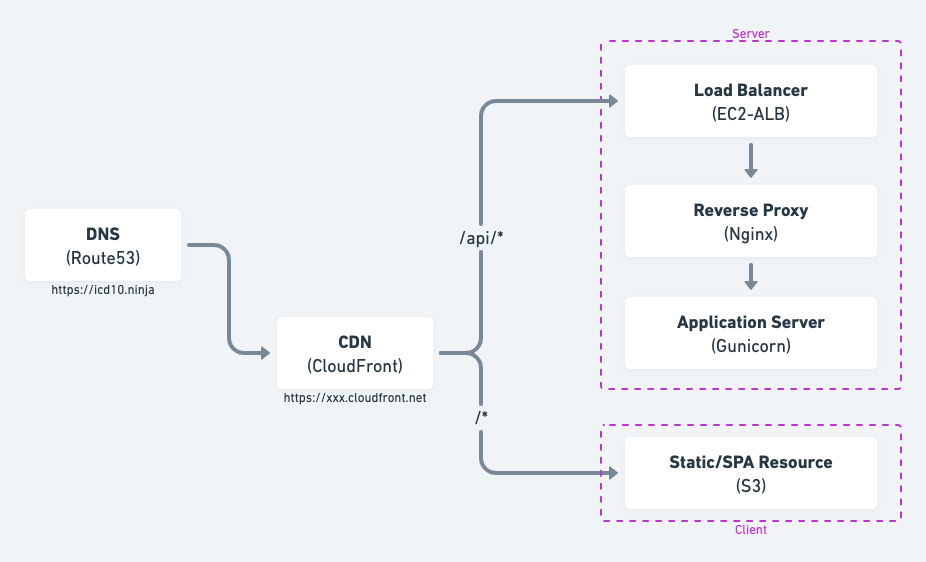
\includegraphics[width=\textwidth]{./images/stack.png}
  \caption{Our model and its client-facing interface in Amazon Web Services (AWS)}
  \label{fig:deployment}
\end{figure}
`
% -------------------------------------------------------------

\newpage
\subsection{Model Interaction via Web Interface} \label{appendix:websitescreenshots}

\begin{figure}[H]
  \includegraphics[width=\textwidth]{./images/website-screenshot-0.png}
  \caption{The Web Application offering choices of exploration to the user}
\end{figure}

\begin{figure}[H]
  \includegraphics[width=\textwidth]{./images/website-screenshot-1.png}
  \caption{Sample results for a \textbf{condition similarity} search for Conjunctivitis}
\end{figure}

\begin{figure}[H]
	\centering
  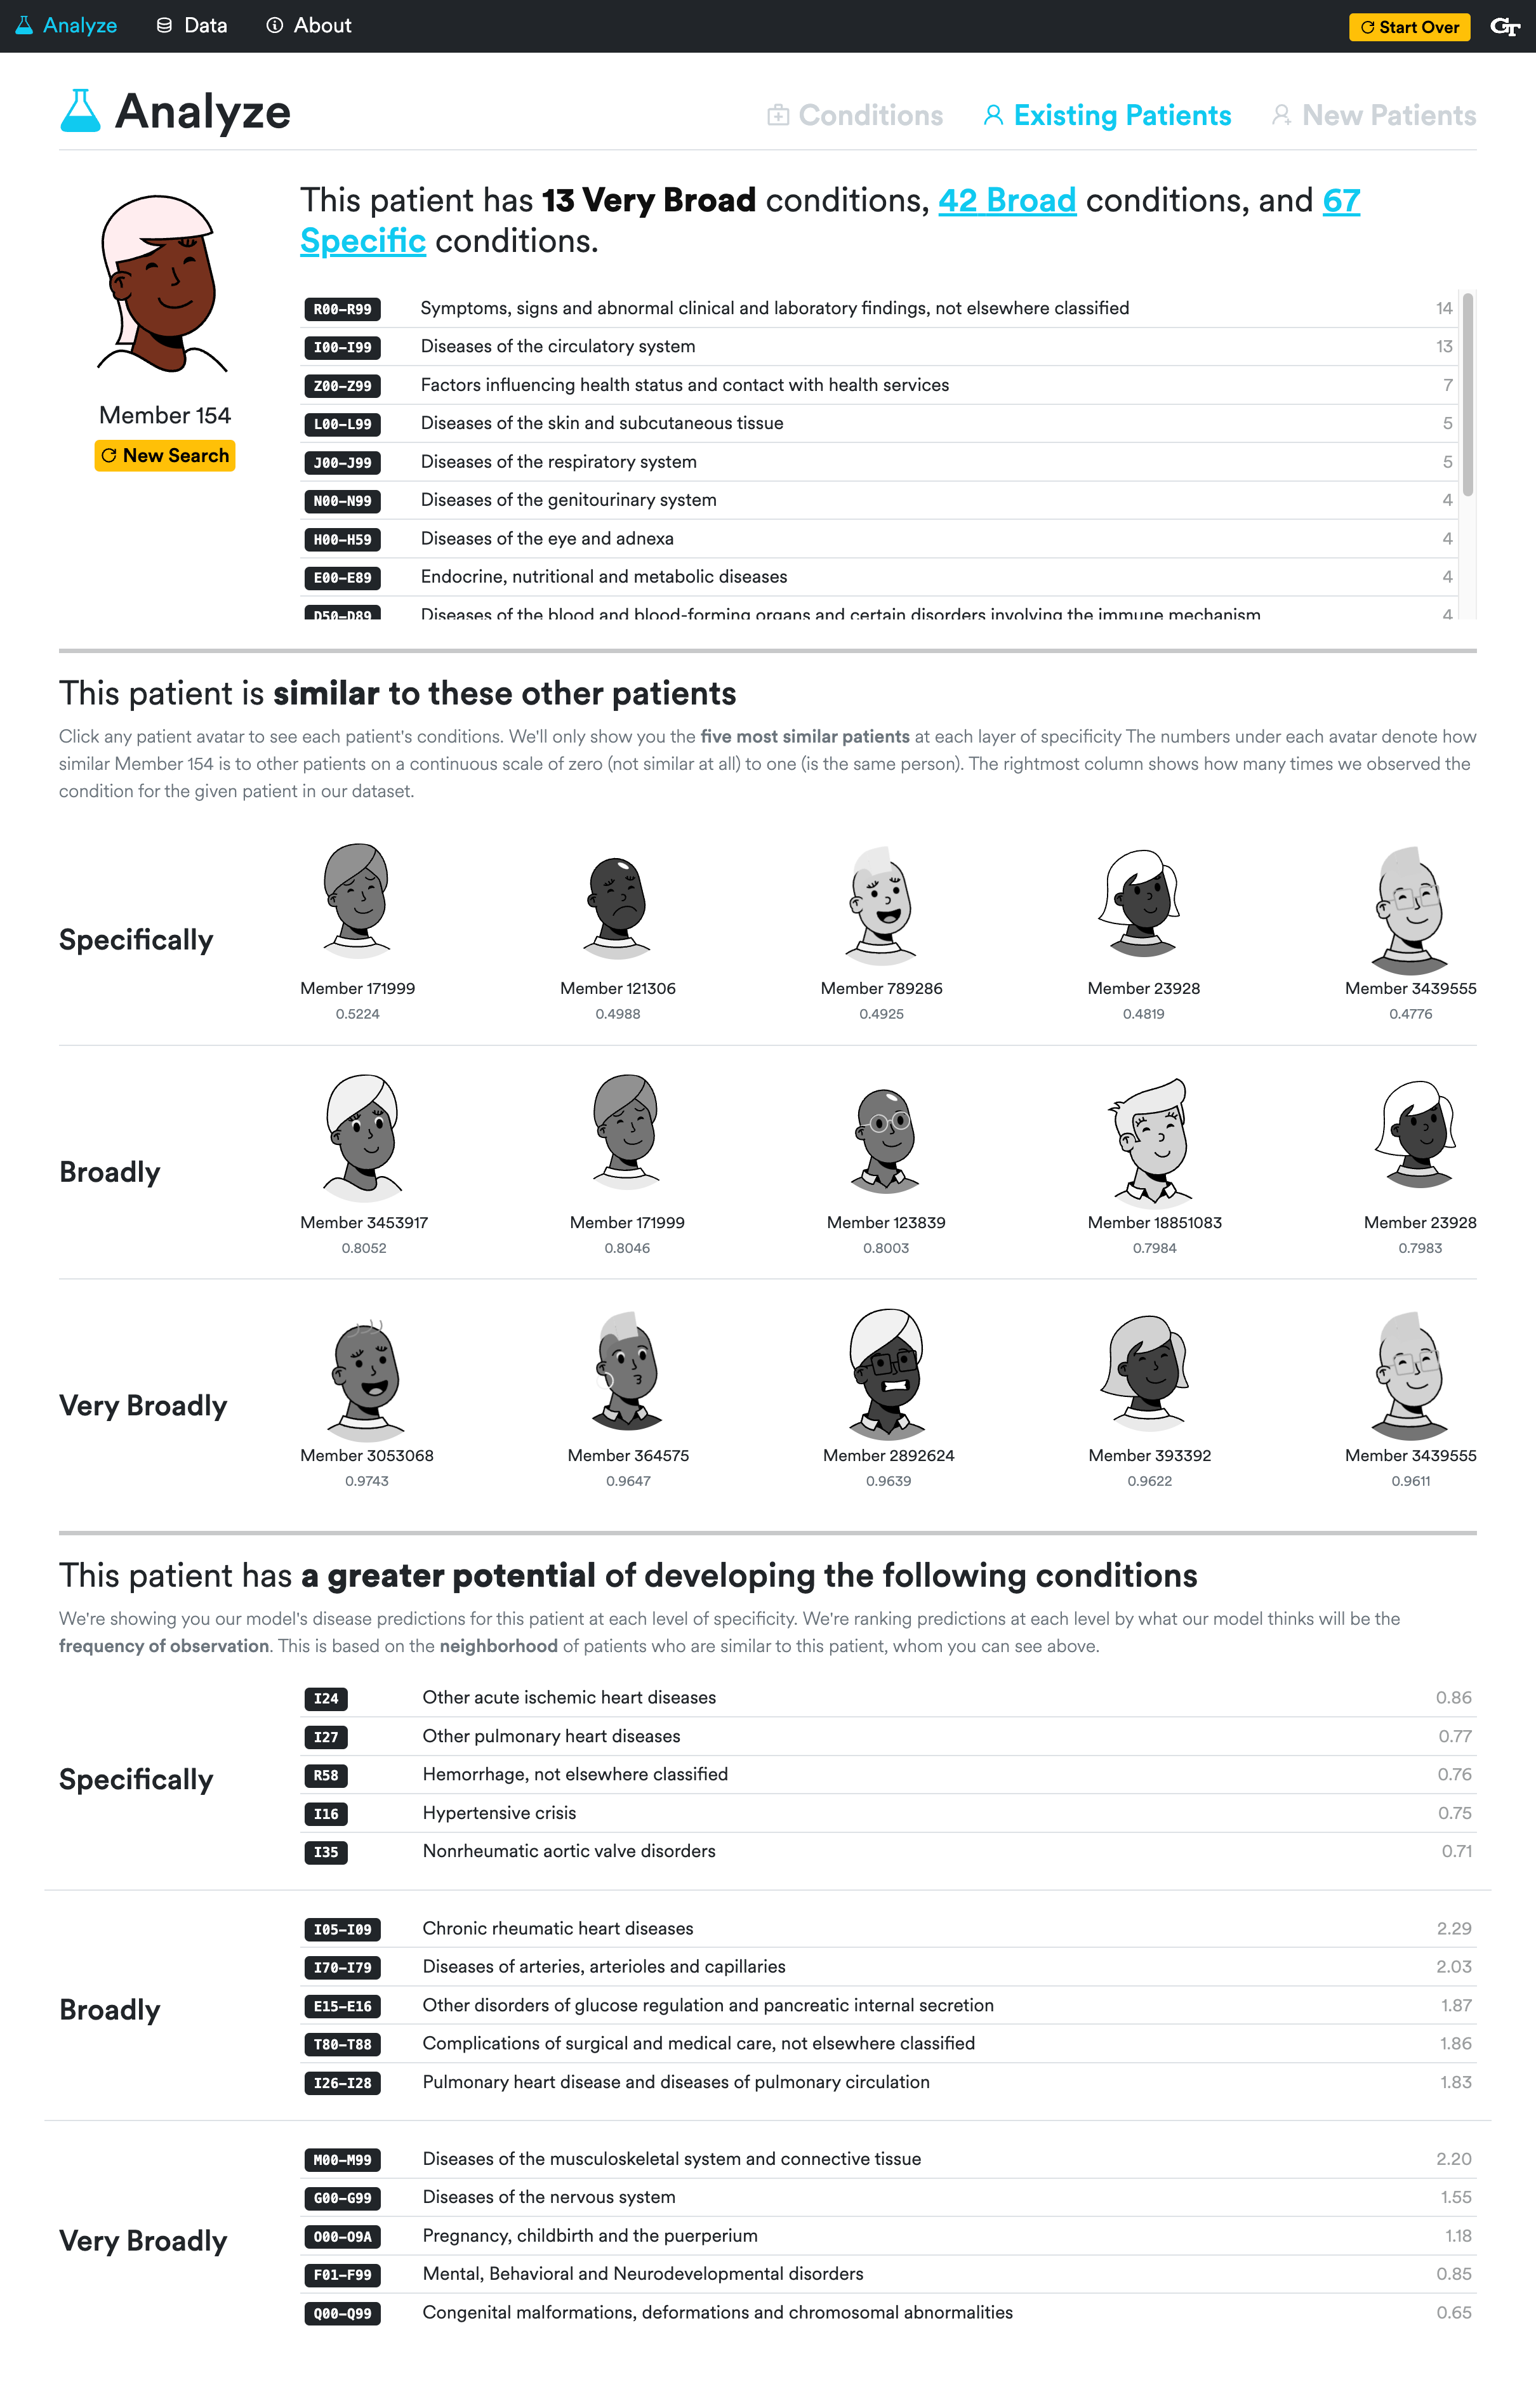
\includegraphics[width=0.8\textwidth]{./images/website-screenshot-existing.png}
  \caption{Sample results for a \textbf{patient similarity} search for a member with ID 154}
\end{figure}

\begin{figure}[H]
	\centering
  \includegraphics[width=\textwidth]{./images/website-screenshot-new-select.png}
  \caption{The web application allowing the creation of a \textbf{new/synthetic patient profile}}
\end{figure}

\begin{figure}[H]
	\centering
  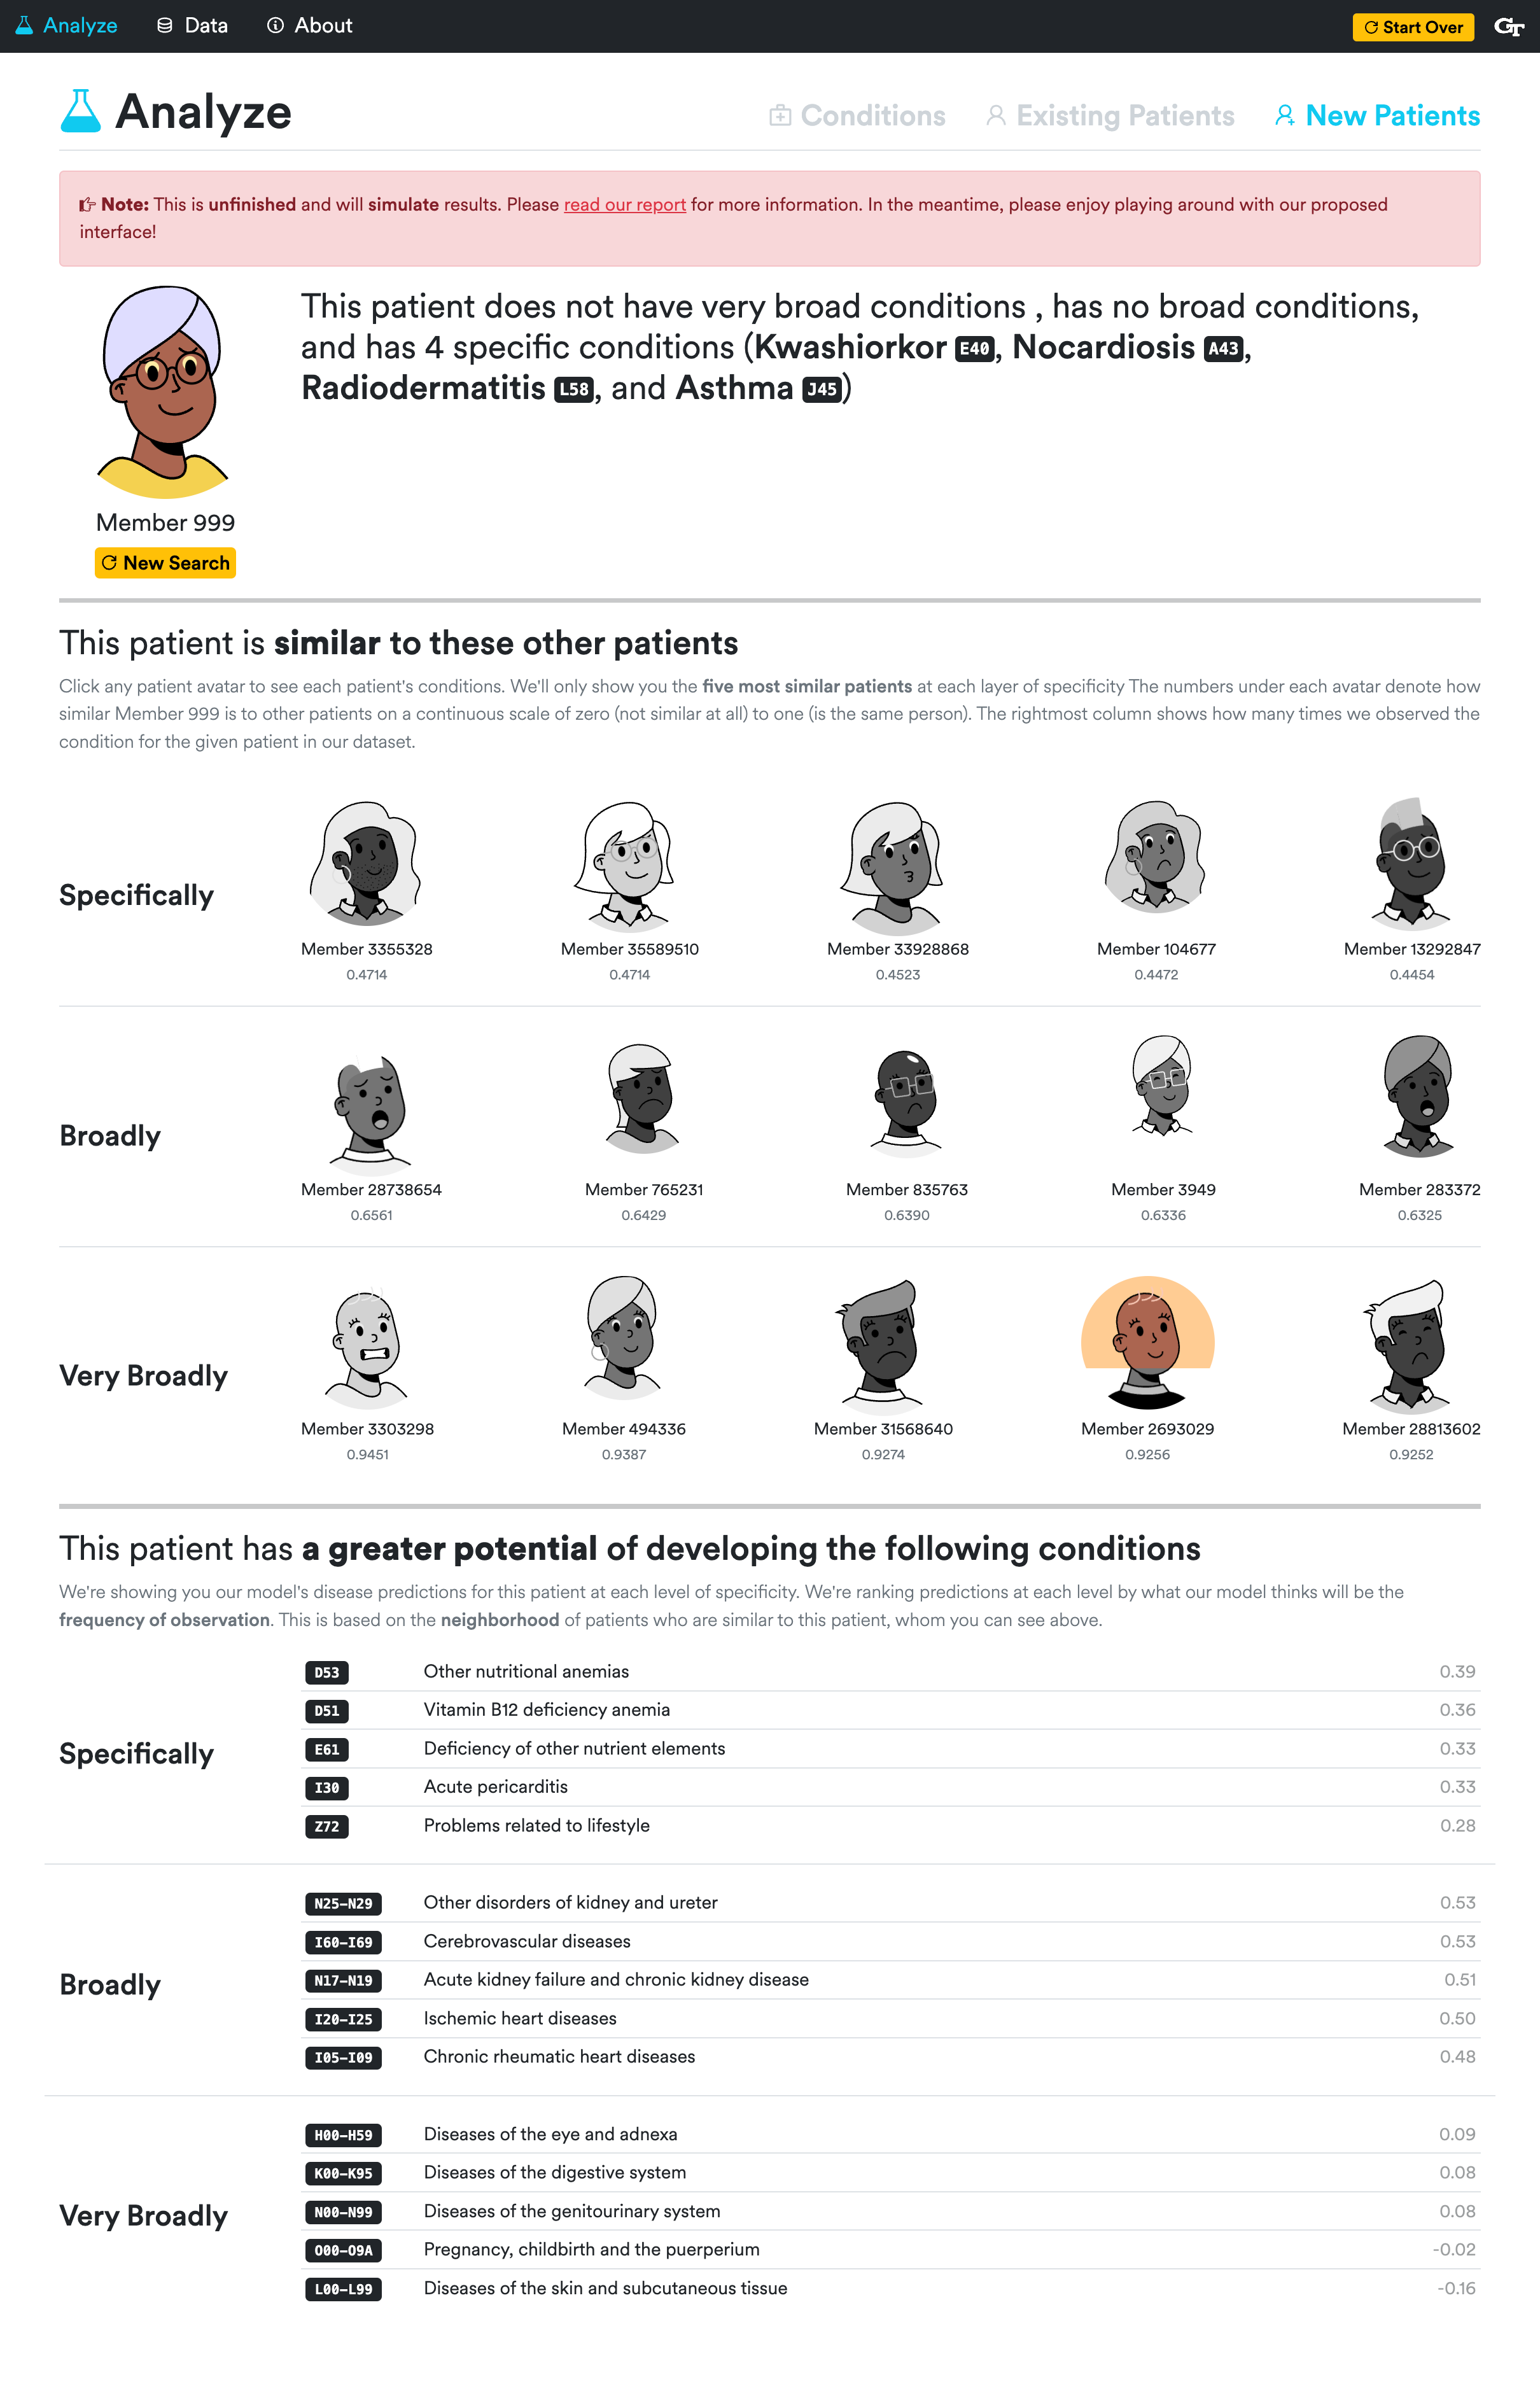
\includegraphics[width=0.8\textwidth]{./images/website-screenshot-new-results.png}
  \caption{Sample results for a \textit{proposed} \textbf{patient similarity} search with a synthetic profile}
\end{figure}

\end{document}



















